\documentclass[../../main.tex]{subfiles}


\begin{document}
\subsection*{(a)}
Import log-flat.xes to ProM. 
Click the eye symbol to view resource. \\
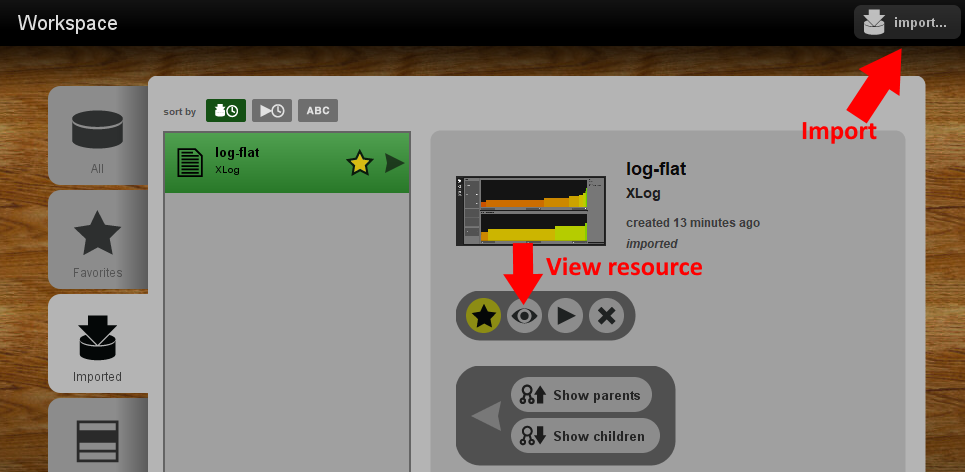
\includegraphics[width=0.8\textwidth]{img/ProM_a_overview.png}\\
This results in the following view:\\
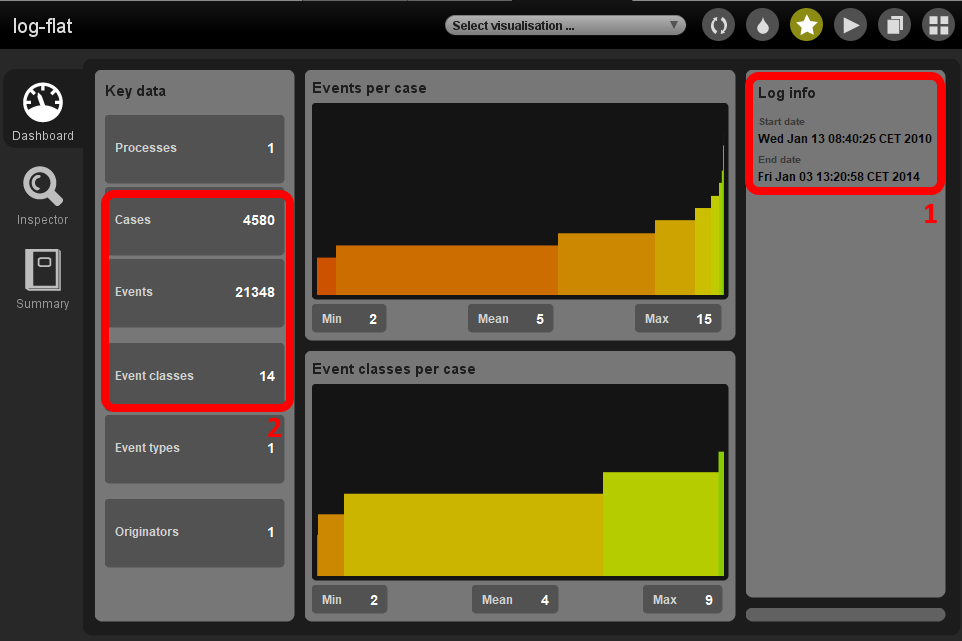
\includegraphics[width=0.8\textwidth]{img/ProM_a_overview_2.png}\\
From it we can read 
\begin{itemize}
\item the time period (1) covered by the event log, which is from 13.01.2010 to 03.01.2014
\item the number of cases, events and activities of the log (2), being 4580, 21348 and 14 respectively (note that activities appear in ProM as event classes)
\end{itemize}
To gain more information on the activities we click the summary tab in the left which results in the following view:\\
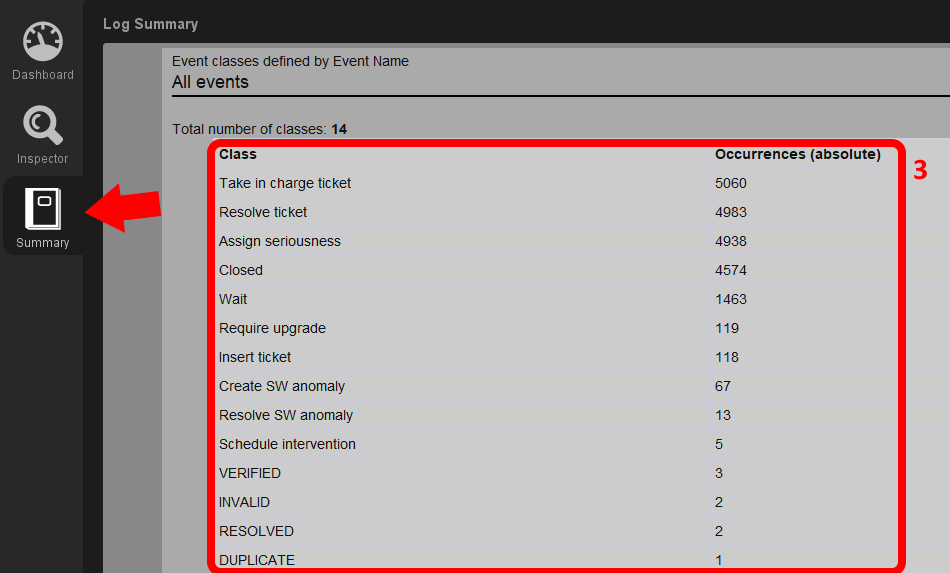
\includegraphics[width=0.8\columnwidth]{img/ProM_a_summary.png}\\
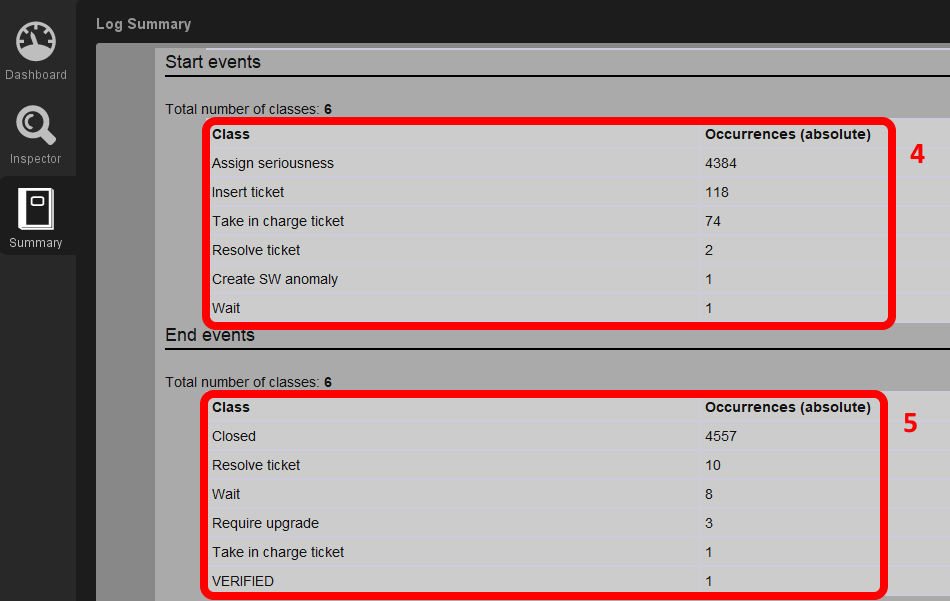
\includegraphics[width=0.8\columnwidth]{img/ProM_a_summary_2.png}\\
From (3) we get a table of occurence frequencies for each activity. From (4) we get a table of occurence frequencies for each start activity. From (5) we get a table of occurence frequencies for each end activity.\\
To determine the number of unique trace variants we click on 'Select visualization' and select 'Explore Event Log'\\
Under this view all trace variants are listed and some further information is given. From this we learn that there are 226 unique variants in the event log.\\
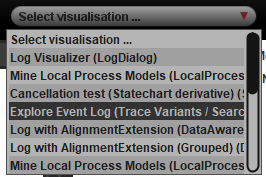
\includegraphics[width=0.5\columnwidth]{img/ProM_a_setting.png}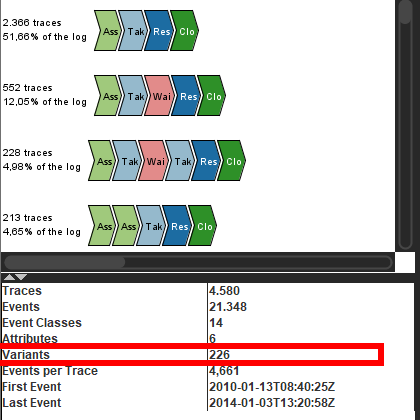
\includegraphics[width=0.5\columnwidth]{img/ProM_a_traces.png}\\

%%%%%%%%%%%%%%%%%%%%%%%%%%%%%%%%%%%%%%%%%%%%%%%%%%%%%%%%%%%%%%%%%%%
98\% of tickets taken in charge are resolved ($\frac{4983}{5060}$)
The variants seem to be quite diverse (\~1:20 ratio of cases to variants, although distributed very unevenly)
%%%%%%%%%%%%%%%%%%%%%%%%%%%%%%%%%%%%%%%%%%%%%%%%%%%%%%%%%%%%%%%%%%%


\subsection*{(b)}
From the introduction we learned that every trace has to start with 'Insert ticket' and ends with 'Closed'. Therefore every trace that does not begin/end with these events must have started/ended outside of our observed time period, making it incomplete.\\
To filter out incomplete traces we go on the 'Actions' tab, select 'Filter Log using Simple Heuristics' and press 'Start'. In the first dialogue we just click 'Next'. In the next dialogue window we select 'Insert ticket' as our only start event and click 'Next'. \\
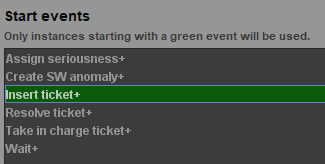
\includegraphics[width=0.5\columnwidth]{img/ProM_b_filter_traces_start.png}\\
For the end events we only select 'Closed' and click 'Next'. \\
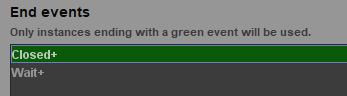
\includegraphics[width=0.5\columnwidth]{img/ProM_b_filter_traces_end.png}\\
Since we do not want to filter out any other events we select 100\% of events in Event Filter and click 'Finish'.\\
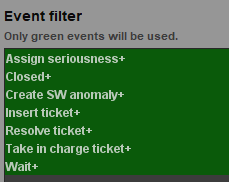
\includegraphics[width=0.5\columnwidth]{img/ProM_b_filter_traces_events.png}\\

\subsection*{(c)}
1. As in (a) we inspect the overview of \textit{log-complete} to find 114 cases, 655 events and 7 activities. Also just like in (a) we select the visualization 'Explore Event Log' to find out there are 20 unique trace variants.\\ 
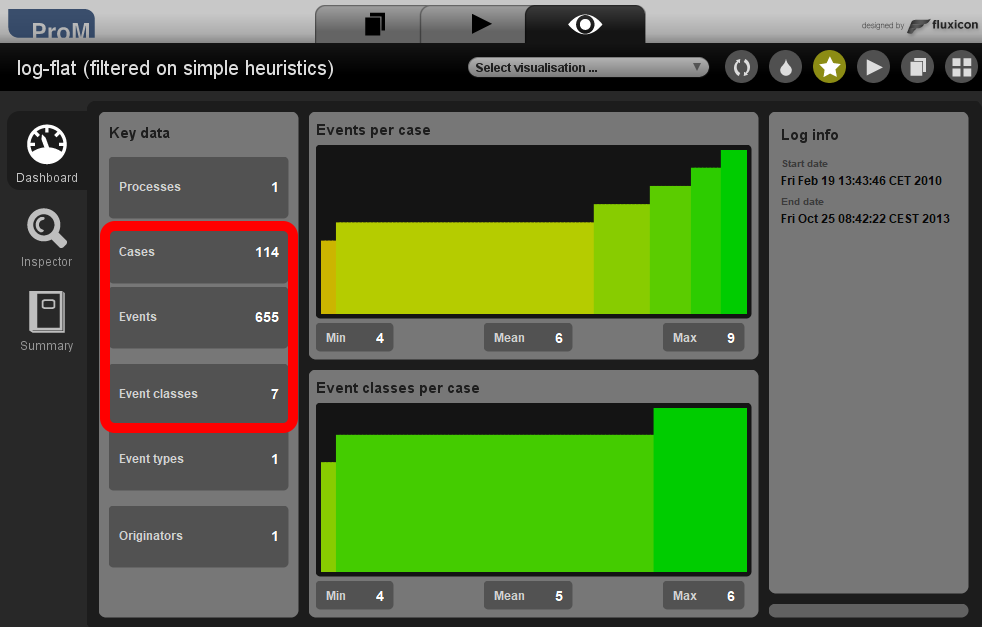
\includegraphics[width=0.6\columnwidth]{img/ProM_c_overview.png}
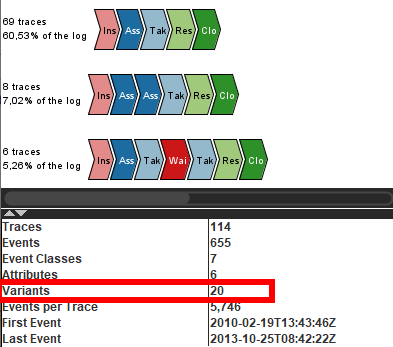
\includegraphics[width=0.4\columnwidth]{img/ProM_c_traces.png}\\
2. Just like in (a) we look at 'Summary' to find a table of activities along with their frequency of occurrence:\\
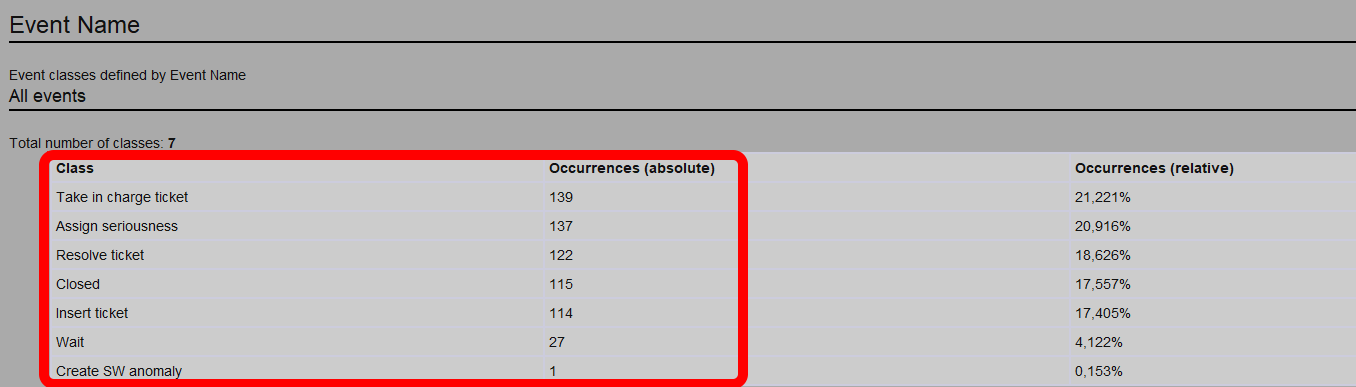
\includegraphics[width=0.8\columnwidth]{img/ProM_c_summary.png}
3.\\
4.\\
5. To find out which activities appear more than once in at least one trace we again take a look at the 'Explore Event Log' visualization:\\
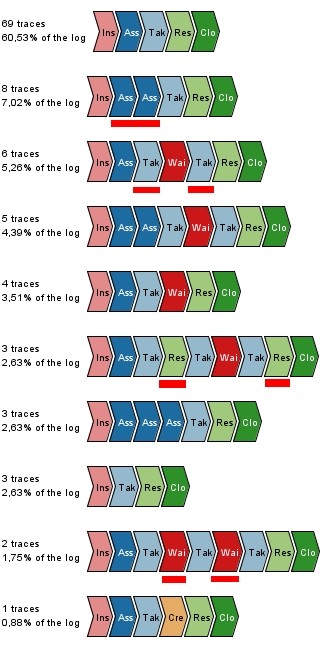
\includegraphics[width=0.5\columnwidth]{img/ProM_c_traces_1.png}
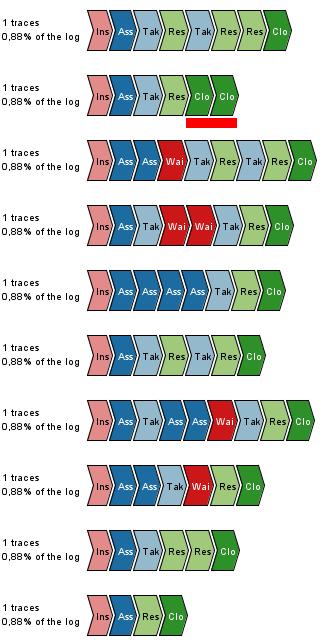
\includegraphics[width=0.5\columnwidth]{img/ProM_c_traces_2.png}\\
The tasks that appear more than once (as marked in the visualization) are
\begin{itemize}
\item Ass: Assign seriousness
\item Tak: Take in charge ticket
\item Res: Resolve ticket
\item Wai: Wait
\item Clo: Closed
\end{itemize}


\subsection*{(d)}
1. We choose Pie Charts for these visualization. For \textit{Ticket type} distribution we choose \texttt{TICKET TYPE} as dimension:
\begin{lstlisting}
"case_table_csv"."TICKET TYPE"
\end{lstlisting} 
and \texttt{COUNT(TICKET TYPE)} as KPI:
\begin{lstlisting}
COUNT("case_table_csv"."TICKET TYPE")
\end{lstlisting} 

For \textit{Membership} distribution we choose \texttt{MEMBERSHIP} as dimension:
\begin{lstlisting}
"case_table_csv"."MEMBERSHIP"
\end{lstlisting} 
and \texttt{COUNT(MEMBERSHIP)} as KPI:
\begin{lstlisting}
COUNT("case_table_csv"."MEMBERSHIP")
\end{lstlisting} 
The resulting distribution visualization can be seen below.\\
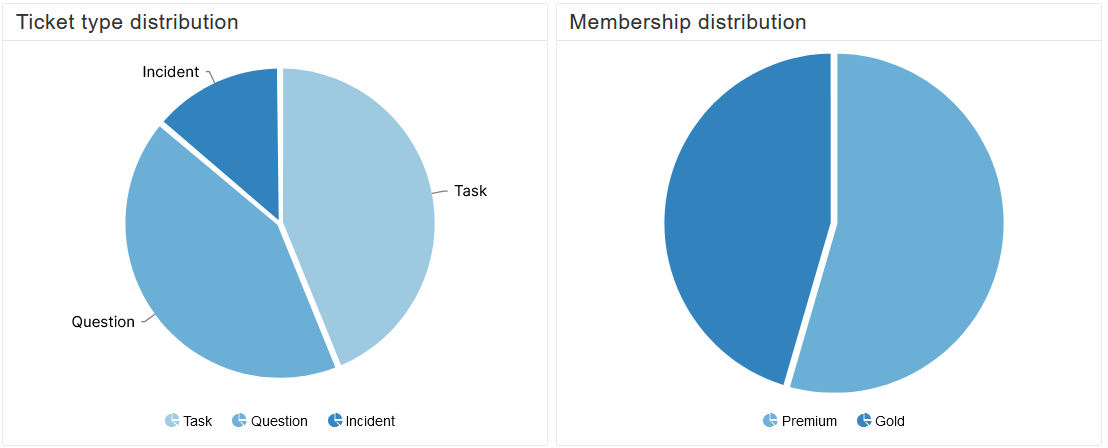
\includegraphics[width=\columnwidth]{img/Celonis_d_ticket_type_and_membership_distribution.png}\\

2. We obtained the column chart titeled 'Total workload per ressource' by using 
\begin{verbatim}
"event_table_csv"."RESOURCE"
\end{verbatim}
as dimension and 
\begin{verbatim}
COUNT("event_table_csv"."ACTIVITY")
\end{verbatim}
as KPI. The x-Axis shows the resources 1-8 in ascending order, the y-Axis shows the summed number of activities handeled by the given resource.

3. We created the column chart named 'Throughput times distribution' by selecting the total throughput time in days as our dimension:
\begin{verbatim}
CALC_THROUGHPUT(ALL_OCCURRENCE['Process Start'] TO ALL_OCCURRENCE['Process End'], REMAP_TIMESTAMPS("event_table_csv"."TIMESTAMP", DAYS))
\end{verbatim} 
and selecting 
\begin{verbatim}
COUNT("case_table_csv"."CASE ID")
\end{verbatim}
as our KPI. The x-Axis shows the throughput time in days and the y-Axis shows the number of cases with a given throughput time.\\
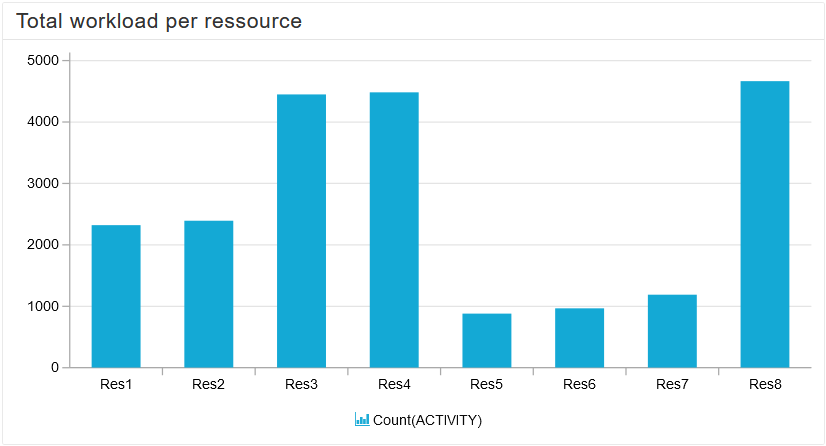
\includegraphics[width=0.5\columnwidth]{img/Celonis_d_workload.png}
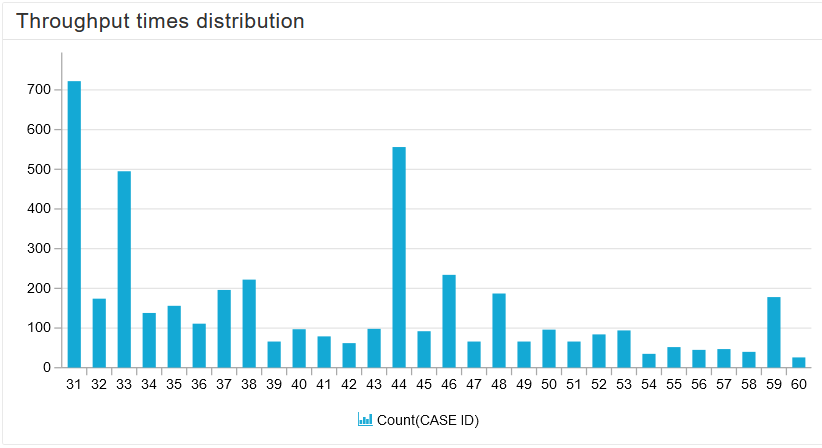
\includegraphics[width=0.5\columnwidth]{img/Celonis_d_throughput_times.png}\\

\end{document}